\documentclass[preview]{standalone}

\usepackage{amsmath}
\usepackage{amssymb}
\usepackage{parskip}
\usepackage{fullpage}
\usepackage{hyperref}
\usepackage{tikz}
\usepackage{stellar}
\usepackage{bettelini}

\hypersetup{
    colorlinks=true,
    linkcolor=black,
    urlcolor=blue,
    pdftitle={Assets},
    pdfpagemode=FullScreen,
}

\begin{document}

\title{Limits}
\id{limits}
\genpage

\section{Definition}

\begin{snippet}{limits-expl1}
A limit is used to describe the behavior of a function as its argument approaches a given value.
The limit towards a certain value \(c\) within a function can be be approached both from the right and from the left.
The limit in a general sense exists if the value approached from both sides is the same and well-defined.
We define the limit of \(x\) approaching \(c\) from the left within the function \(f(x)\) as
\[
    \lim_{x\to c^{-}}f(x)
\]
We define the limit of \(x\) approaching \(c\) from the right within function \(f(x)\) as
\[
    \lim_{x\to c^{+}}f(x)
\]
We define the limit of \(x\) approaching \(c\) within function \(f(x)\) as
\[
    \lim_{x\to c}f(x)
\]
\end{snippet}

\begin{snippet}{limits-definition}
\sdefinition{Limit}{
    Given a function \(f:D\to \mathbb{R}\),
    the limit \[L=\lim_{x\to c}f(x)\] exists if given an arbitrary small
    \(\epsilon >0\) there is another number \(\delta >0\) such that
    \[
        0<|x-c|<\delta
        \implies
        |f(x)-L|<\epsilon
    \]
}
\end{snippet}

\begin{snippet}{limits-definition-illustration}
\begin{center}
    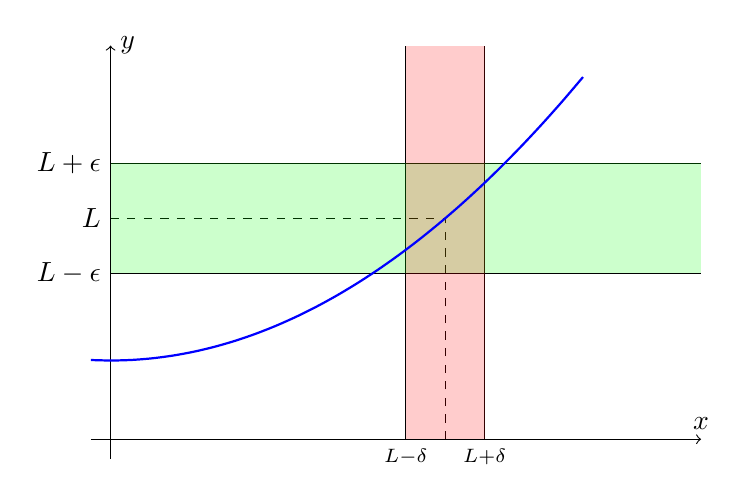
\begin{tikzpicture}[
        declare function={
            func(\x) = \x*\x / 10 + 1;
            LimX=4.25;
            Epsilon=0.7;
            Delta=0.5;
            LimY={func(LimX)};
            Width=7.5;
            Height=5;
        }
    ]
        \draw[->] (0, -0.25) -- (0, Height) node[right] {\(y\)};
        \draw[->] (-0.25, 0) -- (Width, 0) node[above] {\(x\)};

        \draw[-, dashed] (LimX, 0) -- (LimX, LimY);
        \draw[-, dashed] (0, LimY) node[left] {\(L\)} -- (LimX, LimY);

        \draw[-] (0, {LimY + Epsilon}) node[left] {\(L + \epsilon\)} -- (Width, {LimY + Epsilon});
        \draw[-] (0, {LimY - Epsilon}) node[left] {\(L - \epsilon\)} -- (Width, {LimY - Epsilon});

        \draw[-] ({LimX - Delta}, 0) node[below] {\(\scriptstyle L - \delta\)} -- ({LimX - Delta}, Height);
        \draw[-] ({LimX + Delta}, 0) node[below] {\(\scriptstyle L + \delta\)} -- ({LimX + Delta}, Height);

        \fill [green, opacity=0.2] (0,{LimY - Epsilon}) rectangle (Width, {LimY + Epsilon});
        \fill [red, opacity=0.2] ({LimX - Delta}, 0) rectangle ({LimX + Delta}, Height);
   
        \draw[domain=-0.25:6, smooth, variable=\x, blue, thick] plot ({\x}, {func(\x)});
    \end{tikzpicture}
\end{center}
\end{snippet}

\begin{snippet}{limits-expl2}
This means that for any \(x\) in the red region \(0<|x-c|<\delta\text{ or }|x-c|\in (0; \delta)\),
the function at that point will lie in the yellow region.
This value is closer to \(L\) than either \(L + \epsilon\) or \(L - \epsilon\)
\[
    |f(x) - L| < \epsilon
\]
Notice that this defintion does not require \(f\) to be defined at \(c\), but rather just around \(c\).

We can also use this definition for limits from the right and from the left.

The right-hand limit \(L=\lim_{x\to c^{+}}f(x)\) exists if for any arbitrary small \(\epsilon > 0\)
there is some \(\delta > 0\) such that
\[
    |f(x)-L|<\epsilon \text{ when } 0 < x-c < \delta
\]

The left-hand limit \(L=\lim_{x\to c^{-}}f(x)\) exists if for any arbitrary small \(\epsilon > 0\)
there is some \(\delta > 0\) such that
\[
    |f(x)-L|<\epsilon \text{ when } -\delta < x-c < 0
\]
\end{snippet}

\section{Infinite Limits and Limits at Infinity}

\begin{snippet}{right-left-limit-definition}
The limit
\[
    \lim_{x\to c}f(x) = \infty
\]
diverges to \(\infty\) if we can make it arbitrarily large for all \(x\)
sufficiently close to \(c\), without actually letting \(x=a\).
\[
    \forall M \in \mathbb{R} \exists \delta > 0 | f(x) > M \text{ when } 0<|x-a|<\delta, x \neq a
\]
meaning that we can shrink the region around the limit such that its value (expect when \(x=a\))
will always be greater than any number.

The same applies for the limit
\[
    \lim_{x\to c}f(x) = -\infty
\]
where it diverges to \(-\infty\) when
\[
    \forall M \in \mathbb{R} \exists \delta > 0 | f(x) < M \text{ when } 0<|x-a|<\delta, x \neq a
\]
\end{snippet}

\begin{snippet}{vertical-asymptote-limits}
If the limit of a function as it approaches \(a\) diverges,
then it has a vertical asymptote at \(x=a\).
\end{snippet}

\begin{snippet}{horizontal-asymptote-limits}
Limits can approach a value at \(\infty\) or \(-\infty\).
If the limit converges they will have an horizontal asymptote at \(y=L\).
\[
    \lim_{x \to \infty} f(x) = L
    \quad
    \lim_{x \to -\infty} f(x) = L
\]
\end{snippet}

\begin{snippet}{limit-to-inf-convergence}
The limit
\[
    \lim_{x \to \infty} f(x)=L
\]
converges to \(L\) if for every \(\epsilon > 0\) there exists a \(M > 0\) such that
\[
    |f(x)-L| < \epsilon \text{ when } x > M
\]
\end{snippet}

\begin{snippet}{limit-to-inf-convergence-illustration}
\begin{center}
    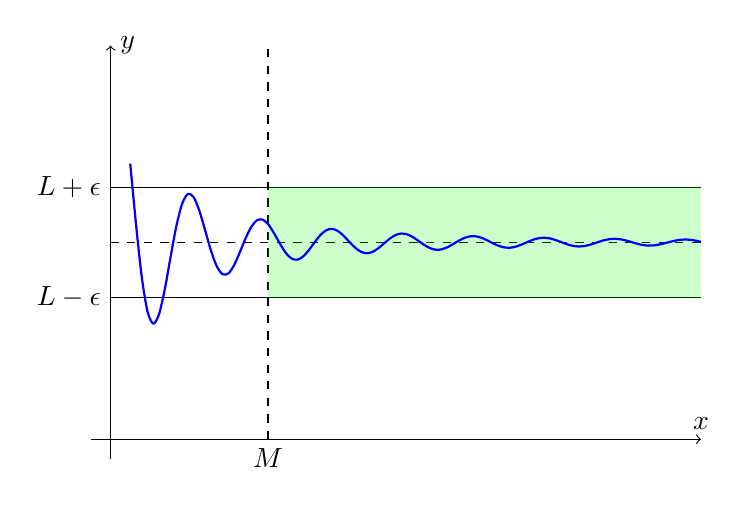
\begin{tikzpicture}[
        declare function={
            L=2.5;
            M=2;
            func(\x) = sin(7 * (\x + 1) r) / (0.4 * (\x + 1) * (\x + 1)) + L;
            Epsilon=0.7;
            Width=7.5;
            Height=5;
        }
    ]
        \draw[->] (0, -0.25) -- (0, Height) node[right] {\(y\)};
        \draw[->] (-0.25, 0) -- (Width, 0) node[above] {\(x\)};
        
        \draw[-, dashed] (0, L) -- (Width, L);
        \draw[-, dashed] (M, 0) node[below] {\(M\)} -- (M, Height);
        
        \draw[-, thin] (0, {L + Epsilon}) node[left] {\(L + \epsilon\)} -- (Width, {L + Epsilon});
        \draw[-, thin] (0, {L - Epsilon}) node[left] {\(L - \epsilon\)} -- (Width, {L - Epsilon});
        
        \fill [green, opacity=0.2] (M,{L - Epsilon}) rectangle (Width, {L + Epsilon});
        
        \draw[domain=0.25:Width, samples=100, smooth, variable=\x, blue, thick] plot ({\x}, {func(\x)});
    \end{tikzpicture}
\end{center}
\end{snippet}

\begin{snippet}{limit-to-neg-inf-convergence}
The limit
\[
    \lim_{x \to -\infty} f(x)=L
\]
converges to \(L\) if for every \(\epsilon > 0\) there exists a \(M > 0\) such that
\[
    |f(x)-L| < \epsilon \text{ when } x < M
\]
\end{snippet}

\begin{snippet}{limits-at-infinity-divergence}
Limits at infinities may also diverge to infinities
\begin{align*}
    \lim_{x \to \infty} &= \infty \text{ if } \forall N \exists M > 0 | f(x) > N, x > M \\
    \lim_{x \to \infty} &= -\infty \text{ if } \forall N \exists M > 0 | f(x) < N, x > M \\
    \lim_{x \to -\infty} &= \infty \text{ if } \forall N \exists M > 0 | f(x) > N, x < M \\
    \lim_{x \to -\infty} &= -\infty \text{ if } \forall N \exists M > 0 | f(x) < N, x < M
\end{align*}
\end{snippet}

\section{Properties}

\begin{snippet}{limits-properties}
If the limit exists
\[
    \lim_{x\to c}f(g(x))=f(\lim_{x\to c}g(x))
\]
\[
    \lim_{x\to c}f(x)g(x) = \lim_{x\to c}f(x) \lim_{x\to c}g(x)
\]
\[
    \lim_{x\to c}f(x)\pm g(x) = \lim_{x\to c}f(x) \pm \lim_{x\to c}g(x)
\]
\[
    \lim_{x\to c}\frac{f(x)}{g(x)} = \frac{\lim_{x\to c}f(x)}{\lim_{x\to c}g(x)}
\]
\end{snippet}

\section{Squeeze Theorem}

\begin{snippet}{squeeze-theorem}
\stheorem{Squeeze Theorem}{
    Let \(h(x)\), \(f(x)\) and \(g(x)\) be three functions such that
    \(h(x) \leq f(x) \leq g(x)\). \\
    If
    \[
        \lim_{x \to x_0} h(x) = g(x) = L
    \]
    then
    \[
        \lim_{x \to x_0} f(x) = L
    \]
}
\end{snippet}

\section{Continuity}

\begin{snippet}{continuity-definition}
\sdefinition{Continuity}{
    A function \(f\) is \textit{continuous} at a point \(c\) if
    \[
        \lim_{c_0 \to c^+} f(c_0) = \lim_{c_0 \to c^-} f(c_0) = f(c)
    \]
}
\end{snippet}

% definitions for limits at infinities
% https://tutorial.math.lamar.edu/Classes/CalcI/DefnOfLimit.aspx

% https://raw.githubusercontent.com/MassimilianoCEZ/Math/main/IT/3rd_year/Analisi_1/ripasso.pdf

\end{document}